\documentclass[a4paper, 12pt, twoside, ]{report}
%\usepackage[latin1]{inputenc}
\usepackage[utf8]{inputenc}
\usepackage[italian]{babel}
\usepackage[T1]{fontenc}
\usepackage{graphicx}
\usepackage{float}
\usepackage {geometry} %[showframe]
\usepackage[centertags]{amsmath}
\usepackage{amsfonts}
\usepackage{amssymb}
\usepackage{amsthm}
\usepackage{newlfont}
\usepackage{array}
\usepackage{fancyhdr}
\usepackage{tesisty}
\usepackage{lipsum} 
\usepackage{lettrine}
\usepackage[dvipsnames]{xcolor}
\usepackage[hidelinks]{hyperref}
\hypersetup{
    colorlinks=false,
    linkcolor =false,
    }



%-------------------------------
% DEFINIZIONE DEGLI ENVIRONMENT
%-------------------------------

\newtheorem{obs}{Osservazione}[section]
\newenvironment{oss}
    {\begin{obs}\begin{normalfont}}
    {\hfill $\square \!\!\!\!\checkmark$ \end{normalfont}\end{obs}}

\newtheorem{pro}{Problema}[chapter]
\newenvironment{prob}
    {\begin{pro}\begin{normalfont}}
    {\hfill $\spadesuit$ \end{normalfont}\end{pro}}

\newtheorem{teor}{Teorema}[section]
\newenvironment{teorema}
    {\begin{teor}\textit }
    {\hfill  \end{teor}}

\newtheorem{defn}{Definizione}[section]
\newenvironment{de}
    {\begin{defn}\begin{normalfont}}
    {\hfill $\clubsuit$ \end{normalfont}\end{defn}}

%-----------------------------
% CONFIGURAZIONE DELLA PAGINA
%-----------------------------

\hfuzz2pt % Don't bother to report over-full boxes if over-edge is < 2pt

\fancypagestyle{plain}{
\fancyhead{}\renewcommand{\headrulewidth}{0pt} } \pagestyle{fancy}
\renewcommand{\chaptermark}[1]{\markboth{\small CAP. \thechapter \textit{ #1}} {} }
\renewcommand{\sectionmark}[1]{\markright{\small  \thesection \textit{ #1}} {} }
\voffset=-20pt    % distanza tra il limite superiore del foglio e l'intestazione
\headsep=40pt     % distanza  l'intestazione ed il testo del corpo
\hoffset=0 pt     % misura equivalente al margine sinistro
\textheight=620pt % altezza del corpo del testo
\textwidth=435pt  % larghezza del corpo del testo
\footskip=40pt    % distanza tra il testo del corpo ed il pie' di pagina
\fancyhead{}      % cancella qualsiasi impostazione per l'intestazione
\fancyfoot{}      % cancella qualsiasi impostazione per il pie' di pagina
\headwidth=435pt  % larghezza del'intestazione e del pie' di pagina
\fancyhead[R]{\rightmark} \fancyfoot[L]{\leftmark}
\fancyfoot[R]{\thepage}
\renewcommand{\headrulewidth}{0.3pt}   % spessore della linea dell'intestazione
\renewcommand{\footrulewidth}{0.3pt}   % spessore della linea del piedi pagina

\numberwithin{equation}{section}
\renewcommand{\theequation}{\thesection.\arabic{equation}}


 
\begin{document}

%-----------------------------
% FRONTESPIZIO - DATI DA MODIFICARE
%-----------------------------



% \dedicate{Inserire la dedica}

\corso{} 
\titoloTesi{\textsc{TITOLO \\ 
Sottotitolo (facoltativo)}} 
\relatore{prof. Xxxxxx Xxxxxx}
\correlatore{prof. Xxxxxx Xxxxxx}
\autore{\normalsize
\begin{flushright}
Tesi di\\
Xxxxx Xxxxxxx\\
Matricola 11111
\end {flushright}}
\anno{\normalsize Sessione Xxxxxx A.A. 202*/202*}

\baselineskip=25pt
\intestazione

\renewcommand{\baselinestretch}{1.5}

%------------------------------------------------
% INTRODUZIONE E RINGRAZIAMENTI (NON MODIFICARE)
%------------------------------------------------

\fancypagestyle{plain}{
\fancyhead{}\renewcommand{\headrulewidth}{0pt} } \pagestyle{fancy}
\renewcommand{\chaptermark}[1]{\markboth{\small Cap. \thechapter \textit{ #1}} {} }
\renewcommand{\sectionmark}[1]{\markright{\small  \S \thesection \textit{ #1}} {} }
\voffset=-20pt                         % distanza tra il limite superiore del foglio e l'intestazione
\headsep=40pt                          % distanza  l'intestazione ed il testo del corpo
\hoffset=0pt                           % misura equivalente al margine sinistro
\textheight=620pt                      % altezza del corpo del testo
\textwidth=435pt                       % larghezza del corpo del testo
\footskip=40pt                         % distanza tra il testo del corpo ed il pie' di pagina
\fancyhead{}                           % cancella qualsiasi impostazione per l'intestazione
\fancyfoot{}                           % cancella qualsiasi impostazione per il pie' di pagina
\headwidth=435pt                       % larghezza del'intestazione e del pie' di pagina
\fancyhead[R]{\rightmark} \fancyfoot[L]{\leftmark}
\fancyfoot[R]{\thepage}
\renewcommand{\headrulewidth}{0.3pt}   % spessore della linea dell'intestazione
\renewcommand{\footrulewidth}{0.3pt}   % spessore della linea del piedi pagina

\pagenumbering{Roman} \tableofcontents
\newpage

\fancyhead[R]{\rightmark} \fancyfoot[L]{}

\chapter*{Ringraziamenti}

\lipsum[1]
\chapter*{Sommario}
\lipsum[2]



\pagenumbering{arabic}

\fancyhead[R]{Introduzione} \fancyfoot[L]{Introduzione}
\fancyfoot[R]{\thepage}

\include{03_Introduzione}

\fancyhf{} %elimina header/footer vecchi


\fancyhead[R]{\rightmark} \fancyhead[L]{\leftmark}
\fancyfoot[R]{\thepage}





%---------------------
% INCLUSIONE CAPITOLI
%---------------------


\chapter{Primo}
\pagestyle{fancy}


\lipsum[1-2]

\section{Sezione con foto}


\lipsum[15]

\begin{center}

\begin{figure}[h]
   \centering 
 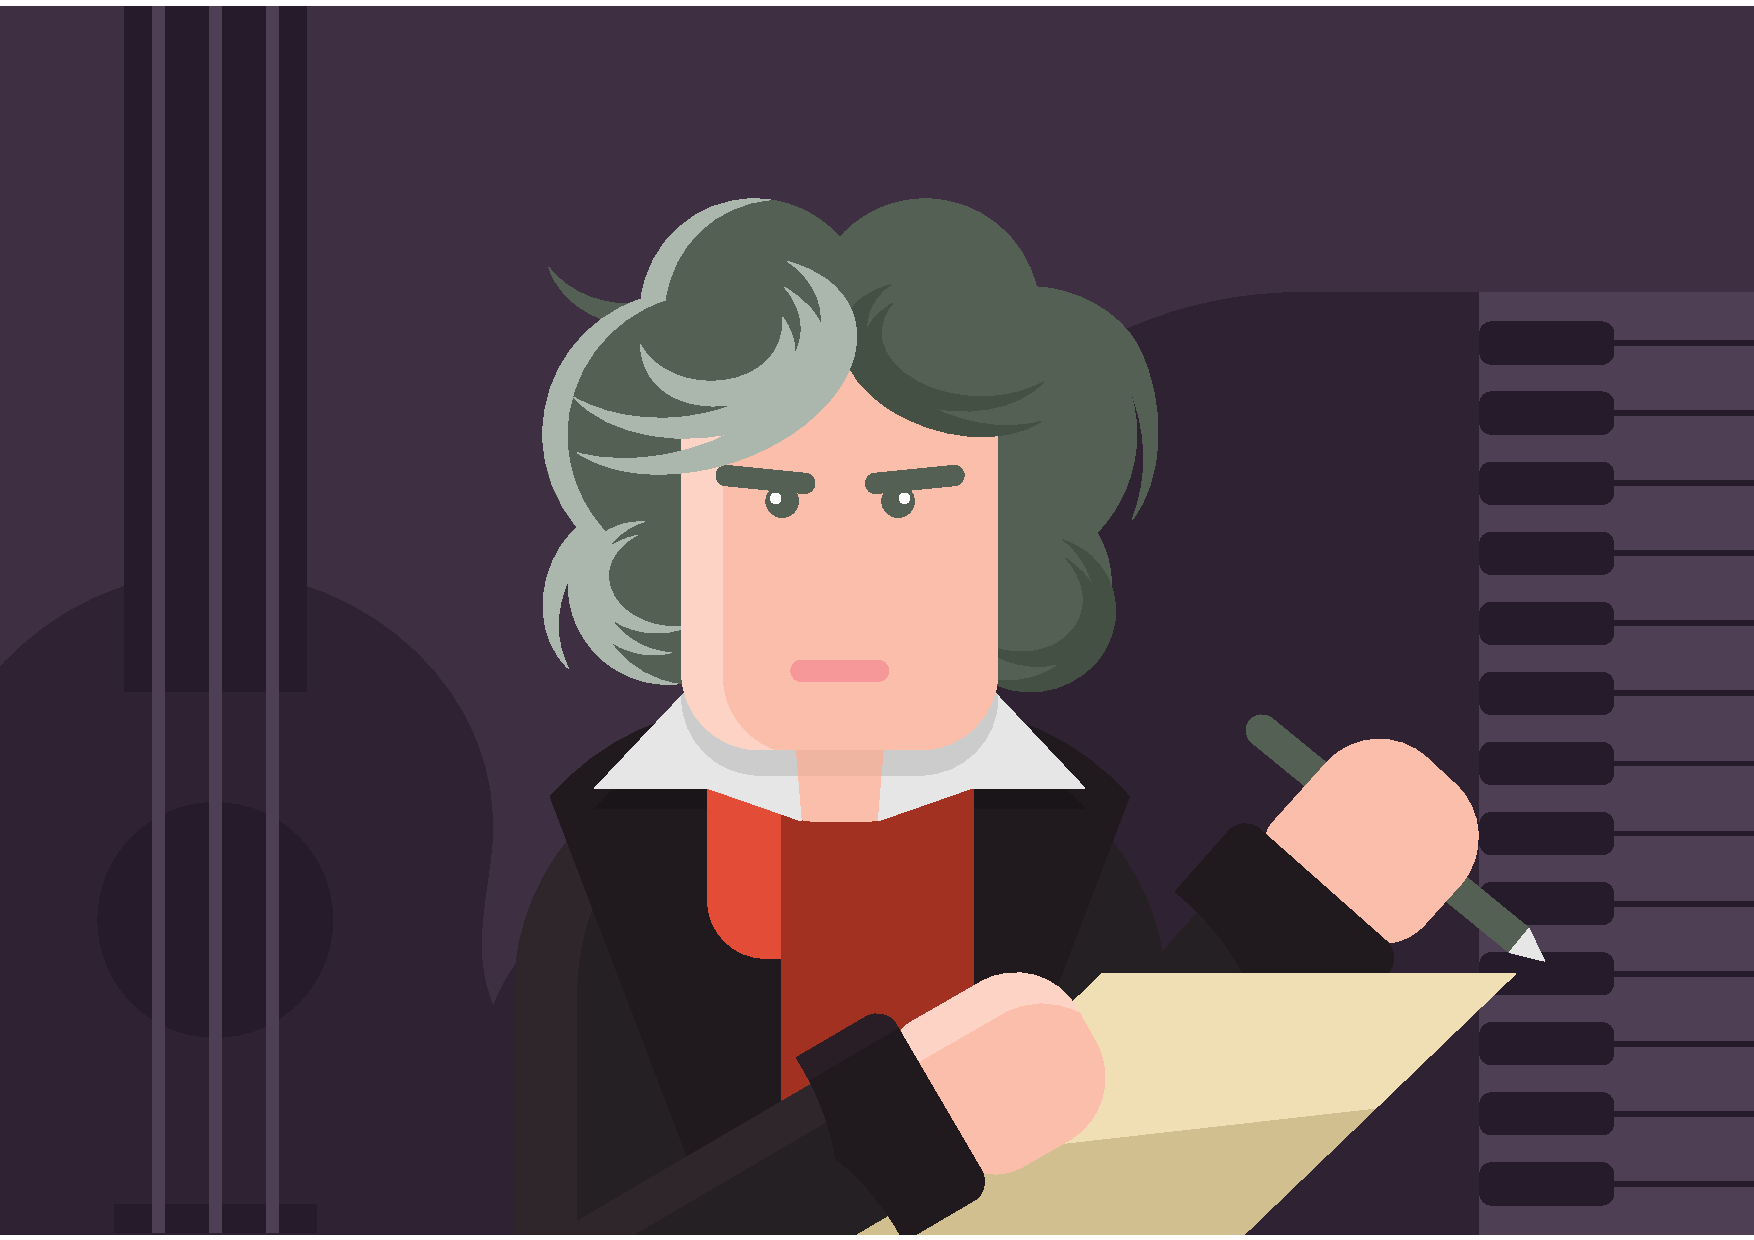
\includegraphics[width=0.7\textwidth]{img/beethoven.pdf}
 \caption{didascalia della foto}
\label{fig: beethoven}
\end{figure}

\end{center}
\chapter{Secondo}
\pagestyle{fancy}




\lipsum[10-12]

\section{Sezione con musica}

\lipsum[13]




\begin{figure}[h]
   \centering 
 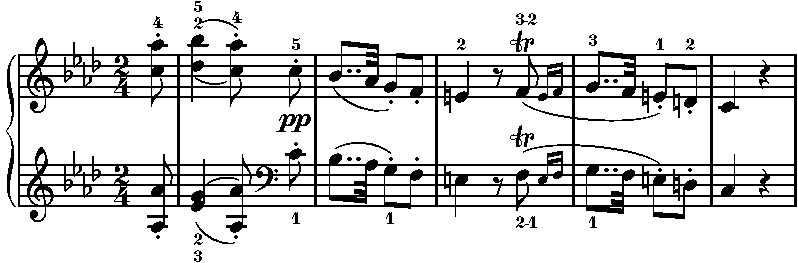
\includegraphics[width=0.9\textwidth]{img/piano.pdf}
\end{figure}



Ecco una nota a pie' di pagina\footnote{Qui si scrive la nota}


\chapter*{Conclusioni}
\addcontentsline{toc}{chapter}{Conclusioni}

\lipsum[1]

% BIBLIOGRAFIA
\addcontentsline{toc}{chapter}{Bibliografia e Sitografia}
\pagestyle{empty}

\begin{thebibliography}{9}
        \bibitem{bib1}\textsc{Cognome}, Nome (data), \emph{Titolo del libro}, Editore, Località (in lingua originale).
        \bibitem{bib2}\textsc{Schell}, Jesse (2014), \emph{The Art of Game Design: A Book of Lenses, Second Edition}, A K Peters/CRC Press, Pittsburgh, Pennsylvania, U.S.A.
     

\vspace*{0.5cm}


\clearpage

        
\noindent \Huge{\textbf{Sitografia}}
\normalsize

\vspace*{0.3cm}
               \bibitem{bib3}\textsc{Nome del sito internet}  \url{https://aaa.com}
        \bibitem{bib4}\textsc{Treccani, il portale del sapere}  -  \url{https://www.treccani.it/enciclopedia}
     
        
        
\end{thebibliography}
\thispagestyle{empty}

\noindent Qui la dichiarazione finale (facoltativa)
\bigskip
 
\noindent\textit{Luogo, Data}

\smallskip

\begin{flushright}
    \begin{tabular}{m{5cm}}
        \\ \hline
        \centering Nome Cognome\\
    \end{tabular}
\end{flushright}





\vspace*{\fill}
\renewcommand{\baselinestretch}{1}

\begin{center}
 \footnotesize{
\textsc {documento rilasciato sotto licenza}}\\

 \begingroup
\noindent ---------------------------------------------------------------------------------------\\
 
\includegraphics[width=3cm]{img/by_nc_sa_eu.png}   \\ 
 \footnotesize{
\textsc{attribuzione non commerciale\\
condividi allo stesso modo - Italia.\\
CC BY-NC-SA 4.0}\\
}
---------------------------------------------------------------------------------------\\

\end{center}
\endgroup








\end{document}
